\documentclass[a4paper]{llncs}
\usepackage{printlen} % Print lengths using specified units. 
\usepackage{booktabs}
\usepackage[utf8]{inputenc} % Umlaute üöä auch normal benutzen und nicht maskieren
% http://www.ctan.org/tex-archive/fonts/ps-type1/cm-super/
\usepackage[T1]{fontenc} % use high quality fonts, please install cm-super
\usepackage[pdftex]{graphicx}
\graphicspath{{./Depictions/}}
\DeclareGraphicsExtensions{.pdf,.jpeg,.jpg,.png}
\usepackage[T1]{url}
\usepackage{listings}
\usepackage[textsize=footnotesize]{todonotes}

\usepackage[
pdftex,
bookmarks=true,
%hidelinks,
unicode=true,
pdfauthor={Sebastian Tramp, Henry Story, Andrei Sambra, Philipp Frischmut, Michael Martin, and S\"oren Auer},
pdftitle={Extending the WebID Protocol with Access Delegation},
pdfkeywords={WebID, Social Semantic Web, Access Delegation}
]{hyperref}

\title{Extending the WebID Protocol with Access Delegation}

\author{Sebastian Tramp\inst{1} \and Henry Story\inst{2} \and Andrei Sambra\inst{3} \and Philipp Frischmuth\inst{1} \and Michael Martin\inst{1} \and S\"oren Auer\inst{1}}

\institute{
Universit\"at Leipzig, Institut f\"ur Informatik, AKSW,\\
Postfach 100920, D-04009 Leipzig, Germany,\\
\email{\{lastname\}@informatik.uni-leipzig.de}\\
\url{http://aksw.org/FirstnameLastname} (WebID)
\medskip\and
Apache Foundation\\ 
\email{henry.story@bblfish.net}\\
\url{http://bblfish.net/people/henry/card\#me} (WebID)
\medskip\and
CNRS Samovar UMR 5157, TELECOM SudParis\\
\email{andrei.sambra@it-sudparis.eu}\\
\url{https://my-profile.eu/people/deiu/card\#me} (WebID)
}

\authorrunning{Sebastian Tramp et al.}

%%%%% LISTINGS
\usepackage{listings} % Typeset source code listings using LaTeX.
% listing styles
\lstset{%
    numberbychapter=false,
    numberblanklines=true,
    numbers=left,
    numberstyle=\tiny,
    basicstyle=\ttfamily\footnotesize,
    emphstyle=\textit,
    tabsize=2,
    framexleftmargin=2pt,
    captionpos=b,
    frame=single,
    breaklines=true
}
\lstdefinestyle{rdf}{morekeywords={}}
\lstdefinestyle{sparql}{
    morekeywords={SELECT,OPTIONAL,FROM,DISTINCT,a,WHERE,FILTER,GROUP,ORDER,LIMIT,BY,IN,AS},
    emph={s,p,o}
}
\lstdefinestyle{turtle}{
    morekeywords={a, @prefix, cert,xsd, foaf, rdf, rdfs, owl},
    morecomment=[s][\textrm]{<}{>},
    morecomment=[s][\textit]{"}{"},
}

\hyphenation{Web-ID}

\begin{document}

\maketitle              % typeset the title of the contribution

\begin{abstract}
The WebID protocol enables the global identification and authentication of agents in a distributed manner by combining asymmetric cryptography and Linked Data.
But in order to decide whether access should be granted or denied to a particular WebID, the authenticating web server may need to retrieve other profiles and linked resources to work out e.g. if the requesting agent is member of an authorized group.
If these linked resources (e.g. FOAF profiles) are required to be publicly available for the server to access it, then this would be a major privacy limitation on a linked Social Network.
In this paper we explore different ways in which an agent can act as a user and we propose an extension to the WebID protocol which allows for delegation of access authorization from a WebID to a third party, e.g. allowing a server to be able to act on behalf of its users.
This extends the range of application scenarios where WebID authentication can be efficiently deployed while increasing privacy.
\end{abstract}

% this prints the current textwidth, so images can be
% generated perfectly fitting to the page (LNCS textwidth: 121.99854 mm)
%\uselengthunit{mm}\printlength{\textwidth}
%\uselengthunit{mm}\printlength{\columnwidth}

\section{Introduction}\label{sec:intro}

The World Wide Web is a peer to peer communication system designed from the outset to work in a global space, between agents distributed around the world and acting in parallel, with no center of control, in a space where new agents can at any point join and there is no complete overview of the whole system.
These agents need know nothing of each other up to the point of their interaction.
This is the force that leads the web to its declarative functional architecture, with its emphasis on naming and a logic of unalterability of the meaning of names (URIs).
  
Agents on the web communicate with each other through a limited number of actions: by making requests for resources (\texttt{GET}), by creating resources (\texttt{POST} or \texttt{PUT}), or even by deleting resources.
Creation or deletion of resources usually require authentication of the agent making the request, and so in many cases do requests for information.

The WebID protocol enables the global identification of agents using asymmetric cryptography in a way that fits cleanly with this architecture:
namely in such a way that agents can verify each others identity without having had any previous interactions and in such a way as to allow trust to build up in a decentralized manner.

A \textit{WebID} is a URI that refers to an agent - person, robot, group or other thing that can have intentions.
The WebID should be a URI which when dereferenced returns a representation whose description uniquely identifies the agent as the controller of a public key~\cite{sporny-m-2011--a,story-h-2009--a}

The WebID protocol is used currently mostly for client authentication%
\footnote{Server authentication using IETF DANE follows much the same logic, except that the lookup for the identity is not done using the HTTP protocol but DNSSEC~\cite{hoffman-p-2012--a}.}.
It is worth noting that the host serving the WebID profiles controls the identity of every agent whose URI is within that server's namespace.
This service is known as the origin server~\cite{barth-a-2011--a}.
It is the origin of all resources served by it. 

We can easily think of the origin server as not only able to respond to requests, but also as an agent able to make requests.
Indeed WebID authentication requires the server to make WebID profile requests to other servers in order to verify the identity of agents making a request to it.
The WebID specification describes this task as being accomplished by a separate agent, the WebID verifier - which could indeed be done by another service on the web (WebID proxy authentication servers).
But it can also be so closely tied to the web service that it would be natural to think of it as part of that same service.
The WebID profile furthermore could be served by the same agent as the one making the request, in which case we have a minimal case of a peer to peer communication.
Note that fetching a WebID profile for WebID authentication should be done anonymously, for fear of authentication deadlocks%
\footnote{For example one can imagine an agent $S$ with profile $P_s$ requesting a resource on server $R$ which requires authentication.
$S$ would send $R$ its certificate, thereby requiring $R$ to dereference $S$'s profile $P_s$ in order to verify the WebID.
If $P_s$ itself requires authentication of $R$ and if $R$ sends a certificate containing a WebID with its profile $P_r$, and if $P_r$ itself requires authentication then it looks like we have a deadlock.}.

Things get more interesting in the authorization space.
Consider a very natural application of WebID: allowing friends of one's friends (FOAF) access to some resources.
This authorization rule will require the web server to fetch each of its users' friends profiles, in order to build up the list of authorised users.
But there is a privacy issue involved here: not everyone wants to make all of their social network publicly visible, and some may not want to make any of it publicly visible.
Those people may then protect their FOAF profile with access control rules such as only allowing FOAF access to it.
How can a server that needs access to these FOAF profiles in order to apply its own access control rules - such as only allowing access to FOAF - get access to the information? 
Would the server itself need to be listed as a FOAF by each of the users friends?
Should the server take on the identity of the user it is fetching resources for? 
How would it be able to do so?
What other solutions are there?
These are the questions we will try to answer in this paper.

The rest of the paper is organized in the following way:
\autoref{sec:req} describes preliminary requirements which we had in mind for our solution,
\autoref{sec:spec} goes into detail with the WebID specification and adds support for authorization delegation,
in \autoref{sec:eval} we describe our reference implementations based on two web applications which is followed by \autoref{sec:relatedwork} where we compare our proposal with two other protocols, namely CORS and OAuth.
Finally, we conclude our work in \autoref{sec:conclusion} and give directions for future work.

%\section{Terminology}
%\textit{Access Delegation} is a relation between two WebID resources.
%The relation describes, under which circumstances a secretary agent has access to a certain resource under the same constraints as the principal agent.
%The secretary agent declares to act in the name of the principal agent.

\section{Preliminary Requirements}\label{sec:req}

%\todo{is this section really needed? It seems mostly to repeat the previous section, and the next one, while loosing the thread of the questioning}

%This section describes several usage scenarios requiring access delegation which can not be solved efficiently with the standard WebID authentication protocol.
%In addition to that, we list derived implementation requirements.

%%\subsection{Basic Use-Cases for Access Delegation} \label{sec:usecases}

%%\subsubsection{Personal Devices and Applications}

%Currently, the default usage intention for WebIDs consists of browser-based authentication scenarios.
%This is an important use-case and should be of special interest since we use the World Wide Web not only through browsers but also through other applications as well as other application on other devices such as smartphones, tablets and freedomboxes\footnote{\url{https://freedomboxfoundation.org/}}.
%In a typical every day usage scenario, we use feed readers and social network clients hand in hand with web browsers.
%All these applications act in the name of their users and fetch and manipulate resources in a way as if it were done by the users themselves and with her browser.
%These applications provide their services to one user only and also run on a device which is commonly accessed by one user only (e.g. a smartphone).
%This class of \textit{private applications} is similar to browsers and can be seen as an extension of the user himself, as argued by Andy Clark and David Chalmers ~\cite{clark-a-1998-7-a}.

%As a slightly different case, we can identify the class of \textit{service applications}.
%These applications also manipulate resources in the name of the user but they do this for more than one user.
%These services are hosted by a third party e.g. not by the user itself, nor by the owner of the protected resource where our user has an interest in.
%In addition to that, we argue that the level of trust which is given by a user is lower than to an application which runs on a personal device and can be turned off by herself.
%A typical application domain for this class of applications is the Social Web, and more specifically, the distributed and semantic Social Web.
%In this infrastructure, multiple services such as photo sharing, recipe management or todo lists create and manipulate artefacts like notes, comments and images and spin a data network based on a Linked Data infrastructure and shared vocabularies~\cite{tramp-s-2012--a}.

%In this paper will show that this class of service applications can not handle access delegation efficiently without an extension to the protocol such as the one we propose.

%\subsubsection{Vacation Replacement}

%I a typical office scenario, employees declare vacation replacements for the time of their holiday in order to achieve an uninterrupted service during that time.

%One option to allow access to the vacation replacement user is to give him the original certificate or to add his private key to the users WebID.
%This solution has two drawbacks: (1) the users certificate is burned after the vacation and she needs to create a new one, (2) a resource guard can not distinguish between the user and the vacation replacement user, which allows for abuse.
%In this context, the principal agent is the employee which is on holiday and her vacation replacement is the secretary agent.

%\subsubsection{Groups and Roles}

%Access for \textit{working groups} to a resource is typically specified in a way that each resource guard needs to maintain an owned or cached list of group members of this group.
%In the Social Semantic Web, these working groups have its own WebID resources which describe the group as an entity and its members as relations to their user WebIDs.
%To authorize a group of agents to access a resource should be as simple as to authorize a single agent.

%In order to allow this, we define the group as the principal agent and all group members as its secretary agents.
%An alternative could be to share one single group certificate with all members or to create a group certificate for each member and describe all public keys in the group WebID.
%Again, these solutions have different drawbacks: (1) a shared certificate needs to be updated each time a user leaves the group, (2) multiple group certificates for each user does not allow for distinguishing which user accessed the resource, which allows for abuse. 
%In this context, the group is the principal agent and all current group members are secretary agents.\todo{A: not sure I agree (see source)}%the group is not an entity, therefore it cannot take actions by iteself. Actions are always performed by users, as part of the group.

%An \textit{office role} is a slightly different construct where a user can access specific resources because of his working description.
%A product manager has access to all product related resources because of her role as product manager and not because of her identity.
%The role itself is identified by a WebID and all access authorization rules should use this WebID instead of a user WebID.

%In this context, the role is the principal agent and the current role owner is the secretary agent.

%\subsection{Implementation Requirements}


In order to make discussion of the problems easier, we distinguish the following roles in the access delegation process:
\begin{enumerate}
    \item The \textit{secretary} acts in the name of another agent, the \textit{principal}.
    \item The \textit{principal} is the agent who has a secretary that acts on its behalf.
\end{enumerate}
The solution we propose will be based on the following general principles:

\paragraph{Distinguish secretary from principal }-
Identity should as far as possible be transparent.
A secretary should have it's own WebID.
The motivation for this is:
(1) It allows resource guards to permit or deny requests based on this information.
(2) Secretary that have many principals do not need to switch their certificate between requests.
(3) It makes it possible to describe the relation between a principal and its secretary using linked data.

\paragraph{Easy to use}-
The one and only place to describe which secretary are allowed to operate for a principal should be the principal's WebID profile.
To grant delegated access to a secretary agent, no other actions than adding 1 triple to the WebID profile should be needed.
Retracting this grant should involve simply removing it from the WebID profile.

%\subsubsection{Linked Data and Read Write Web integration}
%The solution we try to architect aims to enhance the communication for consumption and modification of Linked Data esp. from the applications point of view.
%This means, that existing Linked Data as well as Read-Write-Web principles should not be violated by the architecture.
%\todo{what does rww means here?}

\paragraph{Minimal protocol footprint}-
%In addition to the integration requirement
By using HTTP and working declaratively by placing statements in documents, we make adoption of the delegation easier and avoid complex protocol developments.
We believe that this is a crucial feature of Linked Data in general.

\paragraph{Efficiency}-
Finally, the proposed solution should scale with growing number of users and connections.
In our context this means that an Social Web application should be able to act in the name of thousands of users.

%\subsubsection{No enforcement to reveal agent identities}\todo{maybe we kick this ...}
 
%Since we know that social networks play an important role in a context where communication is restricted by different parties, an 

\section{Extending WebID for Access Delegation}\label{sec:spec}

This section is organized in subsections which build up step by step to the proposed protocol, adding and validating the need at each step for the next one, the final proposed protocol satisfying the previous principles. 

\subsection{Solution 1: Acting as the user}

The simplest solution for any user agent $A$ wishing to act as the user $U$, is for it to create a public/private key pair,  and with the public key thus generated create a certificate $C_u$ with $U$'s WebID in the Subject Alternative Name position and add the public key to the user $U$'s profile $P_u$.
Having done this the agent $A$ can then connect using the certificate $C_u$ and its associated private key, to any service it wishes to, when it wants to work for/as the user $U$.
This has the advantage of requiring no change to the WebID protocol.
It does give the agent $A$ all powers of the user $U$ and so this type of privilege should be limited to agents which are either extensions of $U$ or ones $U$ can or must fully trust anyway.

\lstinputlisting[
    firstline=6,lastline=26,name=webid,style=turtle,float=htb,label=listing:multipleKeyProfile,
    basicstyle=\ttfamily\scriptsize,
    caption={Profile allowing three different agents to act as Romeo}
]{Listings/mutlipleKeys.ttl}

%In addition to the well known User Agents found in browsers on many different devices, there is one agent on which any service requiring WebID authentication trusts implicitly and this is the WebID profile's origin server.
Any server requiring authentication of an agent using WebID must implicitly trust the origin server~\cite{barth-a-2011--a} hosting the WebID profile, since the profile hosting server can change any information in the profile.
%Any user profile can then be thought of as being a user according to the origin server, i.e. \textit{user@origin.org:port} - where \textit{origin.org} is the domain of the origin server, and \textit{port} is the port the server is running on.

When the user owns the origin server and there is a one-to-one relation between the two, as it is the case in a personal FreedomBox\footnote{http://www.freedomboxfoundation.org/}, then the origin server is just an extension of the user, and in that case trusting the server is the same as trusting the user.
%In that case the origin server can in fact just authenticate as the user whenever needed. 

It should be noted that each device can still be distinguished by servers in case of a problem by logging the exact public key that was used to connect to a service. 
It should be possible then to track down which device's private key had been compromised in case of unusual behaviour . 

Things become more interesting when an origin server agent $A$ is serving a number of different profiles $P_1$ \ldots $P_n$ each identifying respectively users $U_1$ \ldots $U_n$ and needs to act on behalf of each of these users.
This would be the situation for company servers, government agencies, educational institutions, charities, football clubs, etc.
This brings up two issues that need to be taken into account, an issue of data perspective and an issue of efficiency. 

\paragraph{Keeping views distinct}-
First whenever $A$ connects as $U_1$ to a remote resource $R$ it has to place the data received in a separate graph from the one it stores public non authenticated data in, and to the one it stores a representation to the same resurce $R$ seen when connected as the different user $U_2$. 
This is because the resource may return different representations depending on who is connecting to it - one representation for close friends of the owner of $R$ perhaps, and one for more distant ones. 
This can be illustrated using N3 graphs, by specifying a relation between a view on a resource (using a yet to be settled on vocabulary), and a graph which is the log:semantics of that view (cf. Listing~\ref{listing:views}). 
It is very important that the agent receiving information from different users not merge the information that was destined to different users, or else information leakage will severely reduce the trust other agents have in that server $A$. 
This requires carefully keeping identified information that was aimed at different users seperate, perhaps by creating different graph stores: one for publically - non authenticated - information, and one graph store for each user the server needs to authenticate as.

\lstinputlisting[
    firstline=8,lastline=36,name=views,style=turtle,float=htb,label=listing:views,
    basicstyle=\ttfamily\scriptsize,
    caption={Views on Juliet's FOAF profile by Freedom Box Laurence, when acting as Romeo and when acting as Lord Montague }
]{Listings/views.n3}

\paragraph{Efficiency}-Secondly, whenever the Origin Server needs to act as $U_1$ to a remote server $R$ it will need to open a new TLS connection to that server using the certificate $C_{u1}$ for that user.
This could require $N$ parallel connections to the same server $S$. 
Opening TLS connections is somewhat expensive, as it requires expensive asymmetric key cryptographic computations. 
When N becomes large, this inefficiency will be perceived as a serious drawback between two organisations.
%\todo{calculate how inefficient this is, and at what size of network this starts really become problematic}
 
\paragraph{Conclusion}

It is possible for any number of software agents to act AS the user by creating themselves a public key as described above.
This does require a very strong trust relation to exist between the agent acting as the user and the user herself, as the two will be mostly indistinguishable in the linked web of trust. 
This method also becomes inefficient the greater the number of different users  an agent is working for.

 
\subsection{Solution 2: Origin Server acting on Behalf of a User}

In order to reduce the number of open connections to any server down to a minimum, it would be useful if the origin server could identify itself directly when making a request and specify on behalf of which of its users it was acting on per request so as to be able to make multiple requests on the same TLS connection.
One way would be for the origin server acting as client to simply use the same public key as the origin server acting as server - that is it could use the same public key as the one used by the TLS server.
It could even use the same certificate.
This would make clear to any server it was connecting to, that it could rely on this server as much as it could on the identity of any resource, and in particular any WebID profiles served by that server.

Still, such an agent connecting to a remote service on behalf of one of its users would then need to identify which user it was acting on behalf of, or the remote service receiving a request would not know which access control rule to apply to the requesting origin server.
For example in our previous example in the Romeo and Juliet story we showed how the Capulet family FreedomBox only shows Juliet as knowing Romeo, when Romeo makes the request on the resource, but not when the request is made by Romeo's father, lord Montague.
That was an easy access control rule for the Capulet FreedomBox to make when the request was using the WebID protocol, since there it would know via the WebID authentication process exactly which identity the user was making the request as. 
But if it is the Origin Server connecting to the Capulet (FreedomBox), identified as their Montague Origin Server, then what representation should the Capulet FreedomBox return? 
Should it return the reduced version available to Lord Montague?
Or should it return the more complete version available to Romeo and his close friends?

The proposal here is for the Origin Server to add to each HTTP request (made over TLS) an \lstinline|On-Behalf-Of| header identifying the user on behalf of which the request is being made with that user's WebID, as shown below:

\begin{verbatim}
GET /juliet/knows HTTP/1.1
Host: capulet.org
On-Behalf-Of: https://montague.net/romeo#me
User-Agent: FreedomBox_FamilyEdition/0.1 
Accept: application/rdf+xml,text/turtle,application/xhtml+xml
\end{verbatim}

The Capulet FreedomBox Guard having verified that this request does indeed come from the origin server of Romeo's profile
\lstinline|<https://montague.net/romeo>| would then be able to accept that since the requesting server could in any case act as Romeo whenever it chose to do so, this protocol making exchange between the Montague and Capulet houses more efficient without making it less secure, this be justification enough for it (the Capulet FreedomBox) to  serve the representation that Romeo would have received had he connected to the server directly.  
In Section~\ref{sec:relatedwork} we will argue that this is very similar to the way CORS deals with access control, namely by adding a header to a request in order to clarify what agent is making the request.

This \lstinline|On-Behalf-Of| header makes it possible for the \textit{secretary} to open only one TLS connection to a remote server and be 
able to specify for each request on behalf of whom it is making it. The Montague FreedomBox could make a request to the Capulet Freedom Box \lstinline|On-Behalf-Of| Romeo, a few milliseconds later \lstinline|On-Behalf-Of| Lord Montague, and so on. 
Again as explained in the previous section it is the responsibility of the Montague FreedomBox to keep the returned information separate, and act with discretion whenever it is acting on behalf of one or the other of the users. 
As such it's role is not unlike the role of Friar Laurence in the play - dedication to people's private matters requires tact and discretion.

\paragraph{Limitations}

Using the same cryptographic key between the server acting as client and as server risks making the keys available to a wider audience, and so increases the risk of key compromise. 
It may be useful if it were possible to decouple the identity of the agent acting on behalf of another user - the \textit{secretary} - from the Origin Server.

%\todo{insert description of On-behalf-Of header (at least the importance of such a feature)}

\subsection{Solution 3: Secretary acting on Behalf of a User}

The origin server acting as a client on behalf of a user can then be thought of as a keeper of secrets for that user.
It should know how to distinguish what remote servers tell it when it is acting on behalf of one user, from what a remote server tells it when it is acting on behalf of another user.
The role of the keeper of secrets for a person is known as the secretary role - a prestigious role taken on for example by figures such as the Secretary of State, Hillary Clinton.

If we now identify the secretary that can act on behalf of a user using a WebID, we can generalise the protocol somewhat.
That is, when an agent - such as the Montague FreedomBox Laurence with WebID \lstinline|<http://montague.net/fb#laurence>| - authenticates to a remote server it can use its own WebID. 
This would allow the \textit{secretary} to have her own public key, and so to reduce the risk of her private key being compromised affecting the server public key.

But how would the remote server know that it can trust that secretary to be acting on behalf of a particular user?
It can no longer just compare the TLS keys of the requesting agent to see if it comes from the same Origin Server.
We need to make this relation explicit by use of a special RDF relation provisionally called \lstinline|:secretary|%
\footnote{A object property with a domain and range as \lstinline|foaf:Agent| which we will provisionally place
in the \lstinline|cert:| namespace, though it may be more appropriately placed in the \lstinline|auth:| namespace.}

%\lstinputlisting[
    %name=schema,style=turtle,float=htb,label=listing:schema,
    %basicstyle=\ttfamily\scriptsize,
    %caption={Schema description of the delegation property},
%]{Listings/schema.ttl}

The remote server can then verify that the identified agent is the secretary of the agent he wishes to act on behalf of (as specified in the \lstinline|On-Behalf-Of| header, by dereferencing that user's profile and verifying that the user specifies the \lstinline|:secretary| relation there, as it would if Romeo had the FOAF profiles as shown in Listing \ref{listing:webid1}.

\lstinputlisting[
    firstline=5,lastline=14,name=webid,style=turtle,float=htb,label=listing:webid1,
    basicstyle=\ttfamily\scriptsize,
    caption={Minimal WebID profile including a public key and a secretary relation}
]{Listings/webid1.ttl}

\begin{figure*}[htb]
  \centering
  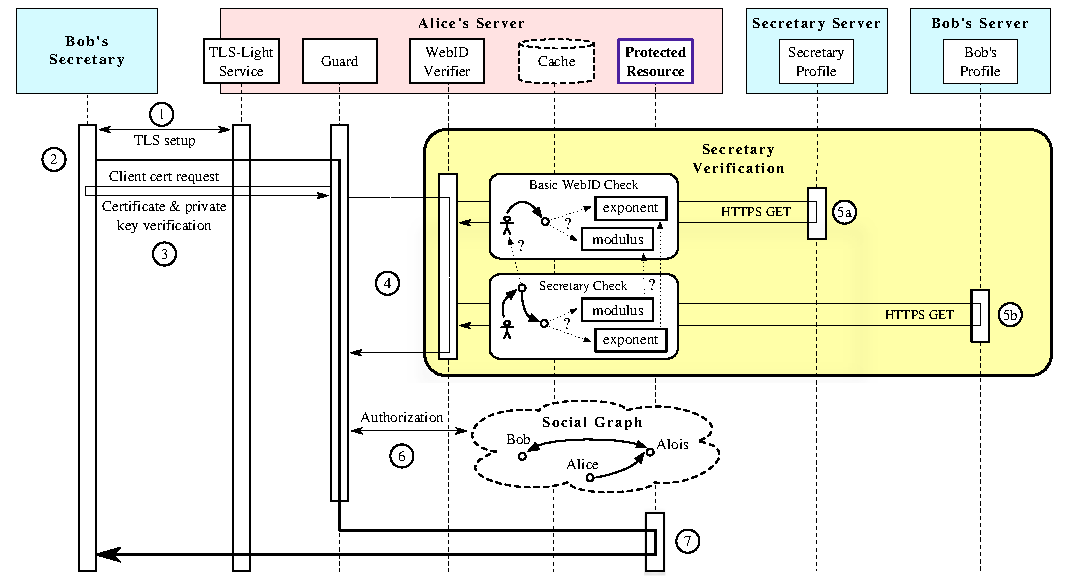
\includegraphics[width=\textwidth]{AuthSequence}
  \caption{Extended WebID authentication sequence}
  \label{fig:AuthSequence}
\end{figure*}

%\autoref{fig:AuthSequence} depicts the process of a WebID authentication which is extended with the following components to allow access delegation:
%\begin{itemize}
    %\item The requesting agent (the secretary) claims a request as requested in the name of a principal agent (see point 2).
        %This adds a HTTP request header to the specification.
    %\item The WebID verifier needs to verify not only one but two different WebID incl. the relation between these two resources (see point 4).
        %This adds additional verification rules to the specification.
    %\item The principal agent (Bob) can declare any relation to his secretary agents in his WebID profile.
        %This adds a vocabulary for describing access delegation to the specification.
%\end{itemize}


%\autoref{fig:AuthSequence} depicts the process of a WebID authentication which is extended with the following components to allow access delegation:
The following enumeration describes each authentication step of \autoref{fig:AuthSequence} in detail but concentrates on the context of access delegation:
(1) The secretary  opens a TLS connection with the server of the protected resource.
(2) Once TLS is set up, the HTTP request is sent to the server (e.g. a \verb!HTTP GET!), with an additional \lstinline|On-Behalf-Of| header, which thereby defines the requesting agent as a \textit{secretary} and the referred to agent as the \textit{principal} 
(3) The guard intercepts this request, and  in turn requests client authentication using TLS session renegotiation.
The \textit{secretary} authenticates as itself by sending a Certificate containing a WebID refering to it. The TLS-Light service verifies that the \textit{secretary} really is in possession of the private key corresponding to the public key sent in the certificate.
This is defined in the TLS protocol \cite{dierks-t-2012--a}.
(4) The guard ask the verification agent to verify the secretary WebID which is named in the certificate (5a).
This process is exactly as described in the WebID protocol~\cite{story-h-2009--a}.
The guard also asks the verifier agent to check the secretary claim implied by the \lstinline|On-Behalf-Of| header.
(5b) The \textit{principal} agent's relation to the \textit{secretary} is  verified by dereferencing the \textit{principal}'s WebID Profile, and verifying it responds with a true to the SPARQL ASK query \lstinline|ASK { ?principal :secretary ?secretary . }| where the \lstinline|?principal| and \lstinline|?secretary| variables have been bound to the correct URIs.
(6) The authentication and verification process having succeeded, the authorization process checking if the \textit{principal} would get access to the requested resource.
(7) The resource representation can then be returned or not depending on the access control rules.

%\lstinputlisting[
    %firstnumber=last,firstline=13,name=webid,style=turtle,float=htb,label=listing:webiddelegation,
    %basicstyle=\ttfamily\scriptsize,
    %caption={Access delegation by explicitly and implicitly identifying agents or application},
    %label={list:sec_relation},
%]{Listings/webid1.ttl}\todo{A:why add the public key of the agent here? (revocation issues)}

\section{Implementation and Evaluation}\label{sec:eval}

As two real-world examples we describe two different implementations where WebID delegation is deployed and needed.
MyProfile is WebID profile service application and OntoWiki a semantic data wiki.

\textbf{MyProfile}\footnote{\url{http://myprofile-project.org/}}
is a web server demonstrating how easy it is to create a WebID profile, and buidling up some distributed social web applications upon this.
Its main purpose is to provide a unified user account, or simply \textit{user profile}. Currently these are tied to the my-profile-project web site, but it has been architected from the ground up to  work with distributed linked data, making it then easy to dissociate the software stack from the myprofile-project domain name,  and allowing it to be deployed on a machine under the user's control, prefereably even a device located within the user physical reach.


%\begin{figure*}[htb]
  %\centering
  %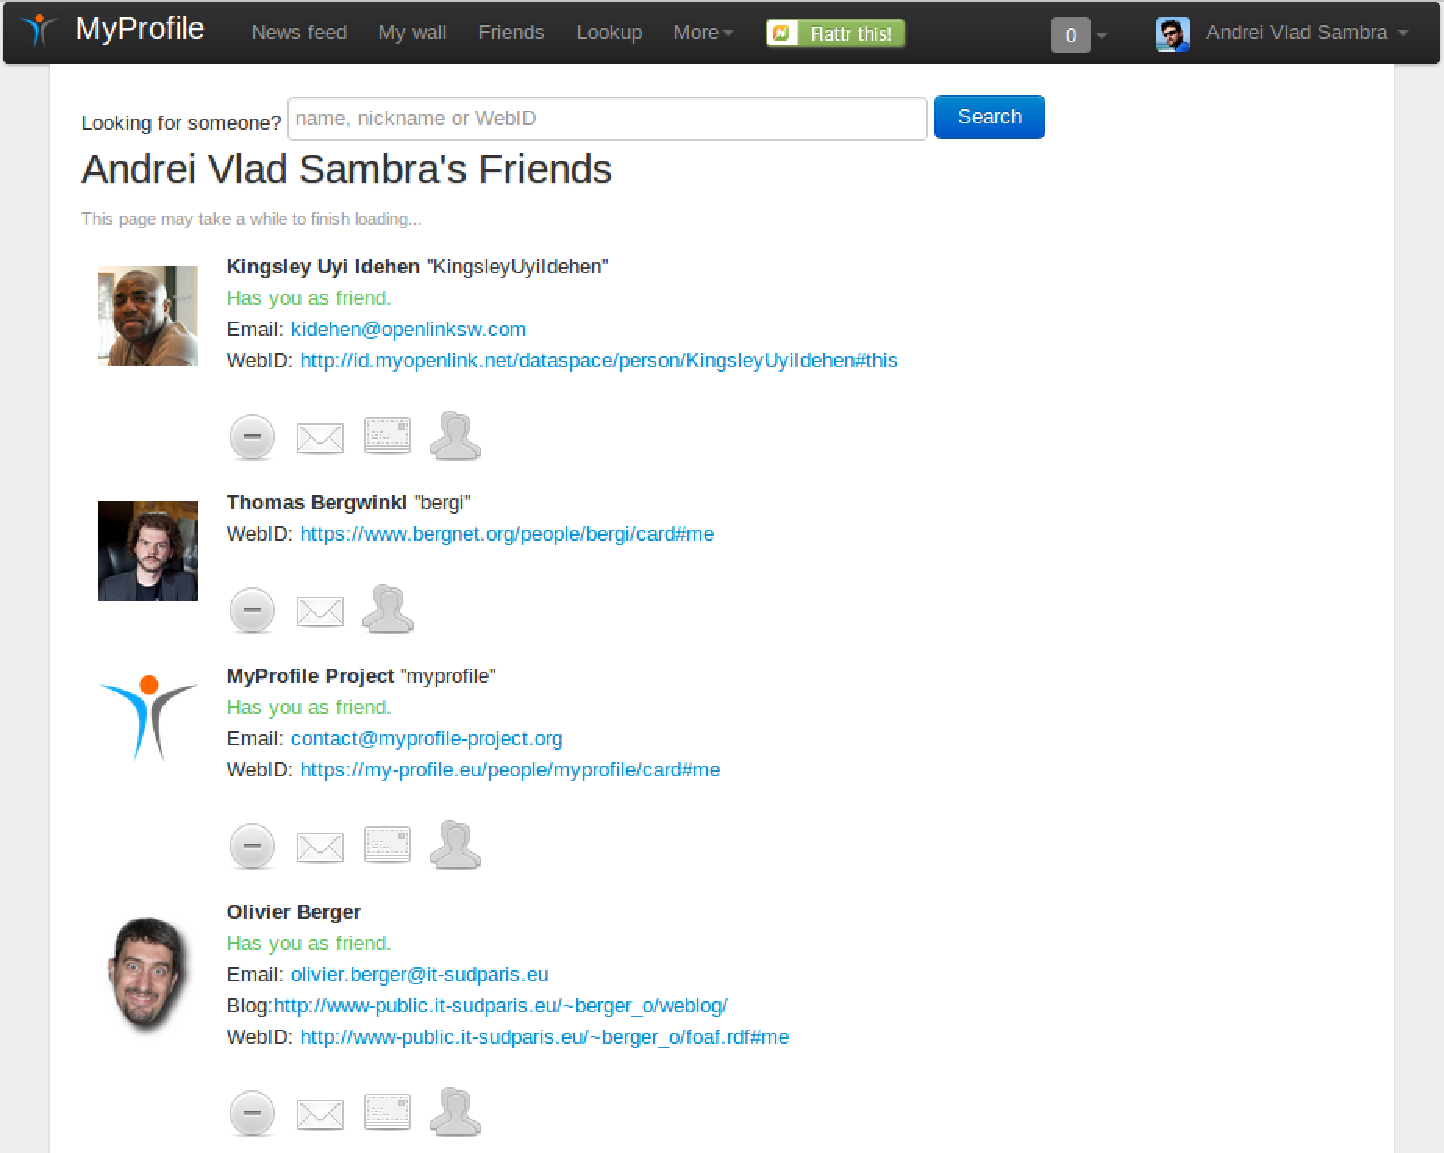
\includegraphics[width=\textwidth]{myprofile}
  %\caption{The MyProfile dashboard visualizes information from different sources fetched by the MyProfile server as a secretary for its users}
  %\label{fig:myprofile}
%\end{figure*}

In the case of MyProfile, it is very important to be able to offer WebID access delegation, because a single MyProfile server instance can host multiple users, and must fetch resources for each user asynchronously in order to be able to provide a seamless and rapid user experience.
To improve user experience and overall performance, a caching mechanism is used to refresh local copies or "views" of external data.
Due to multiple users coexisting on the same server, the caching mechanism needs to be able to distinguish views of remote resources as seen by different users, as they are served by remote servers depending on their access control and resoure filtering policies.

Let's take for example the following case:
Ann and Barry are both local users on a single MyProfile server.
Charley is an external user with access control policies set up on his private server.
When Ann requests to view Charley's profile data, a personalized view of the profile is displayed, corresponding to access control policies by Barry for requests made by Ann.
When Barry requests to view Charley's profile, different profile data is displayed, since there are different access control policies for Barry.
The caching mechanism needs to be able to cache two different profile views, each corresponding to access control policies specific for the user requesting the data.
As the number of users on MyProfile grows this has to be done as efficiently as possible, and so re-using TLS connections where possible is a laudable aim.

\textbf{OntoWiki}
\cite{auer-s-2006-736-a} is a web application, which allows publication, exploration as well as manipulation of arbitrary RDF knowledge bases in distributed scenarios.
We refer to it as a data wiki, since it adopts the wiki philosophy (ease of editing, tracking of changes, integrated discussions) on the one hand, while focussing on structured information on the other hand.
Furthermore OntoWiki is an adaptable application framework, which supports the creation of Linked Data based applications on the web~\cite{heino-n-2009-61-a}.
In addition to the usual features of wikis, OntoWiki provides a sophisticated extension system, such that it can be adapted for a variety of use-cases.
Although the wikis usually enable anyone to edit everything, numerous real-world applications require aaccess-control mechanisms.
OntoWiki has built-in support for authorization on graph and action level.
Furthermore several authentication protocols can be employed, including amongst others the WebID protocol.

%\begin{figure*}[htb]
  %\centering
  %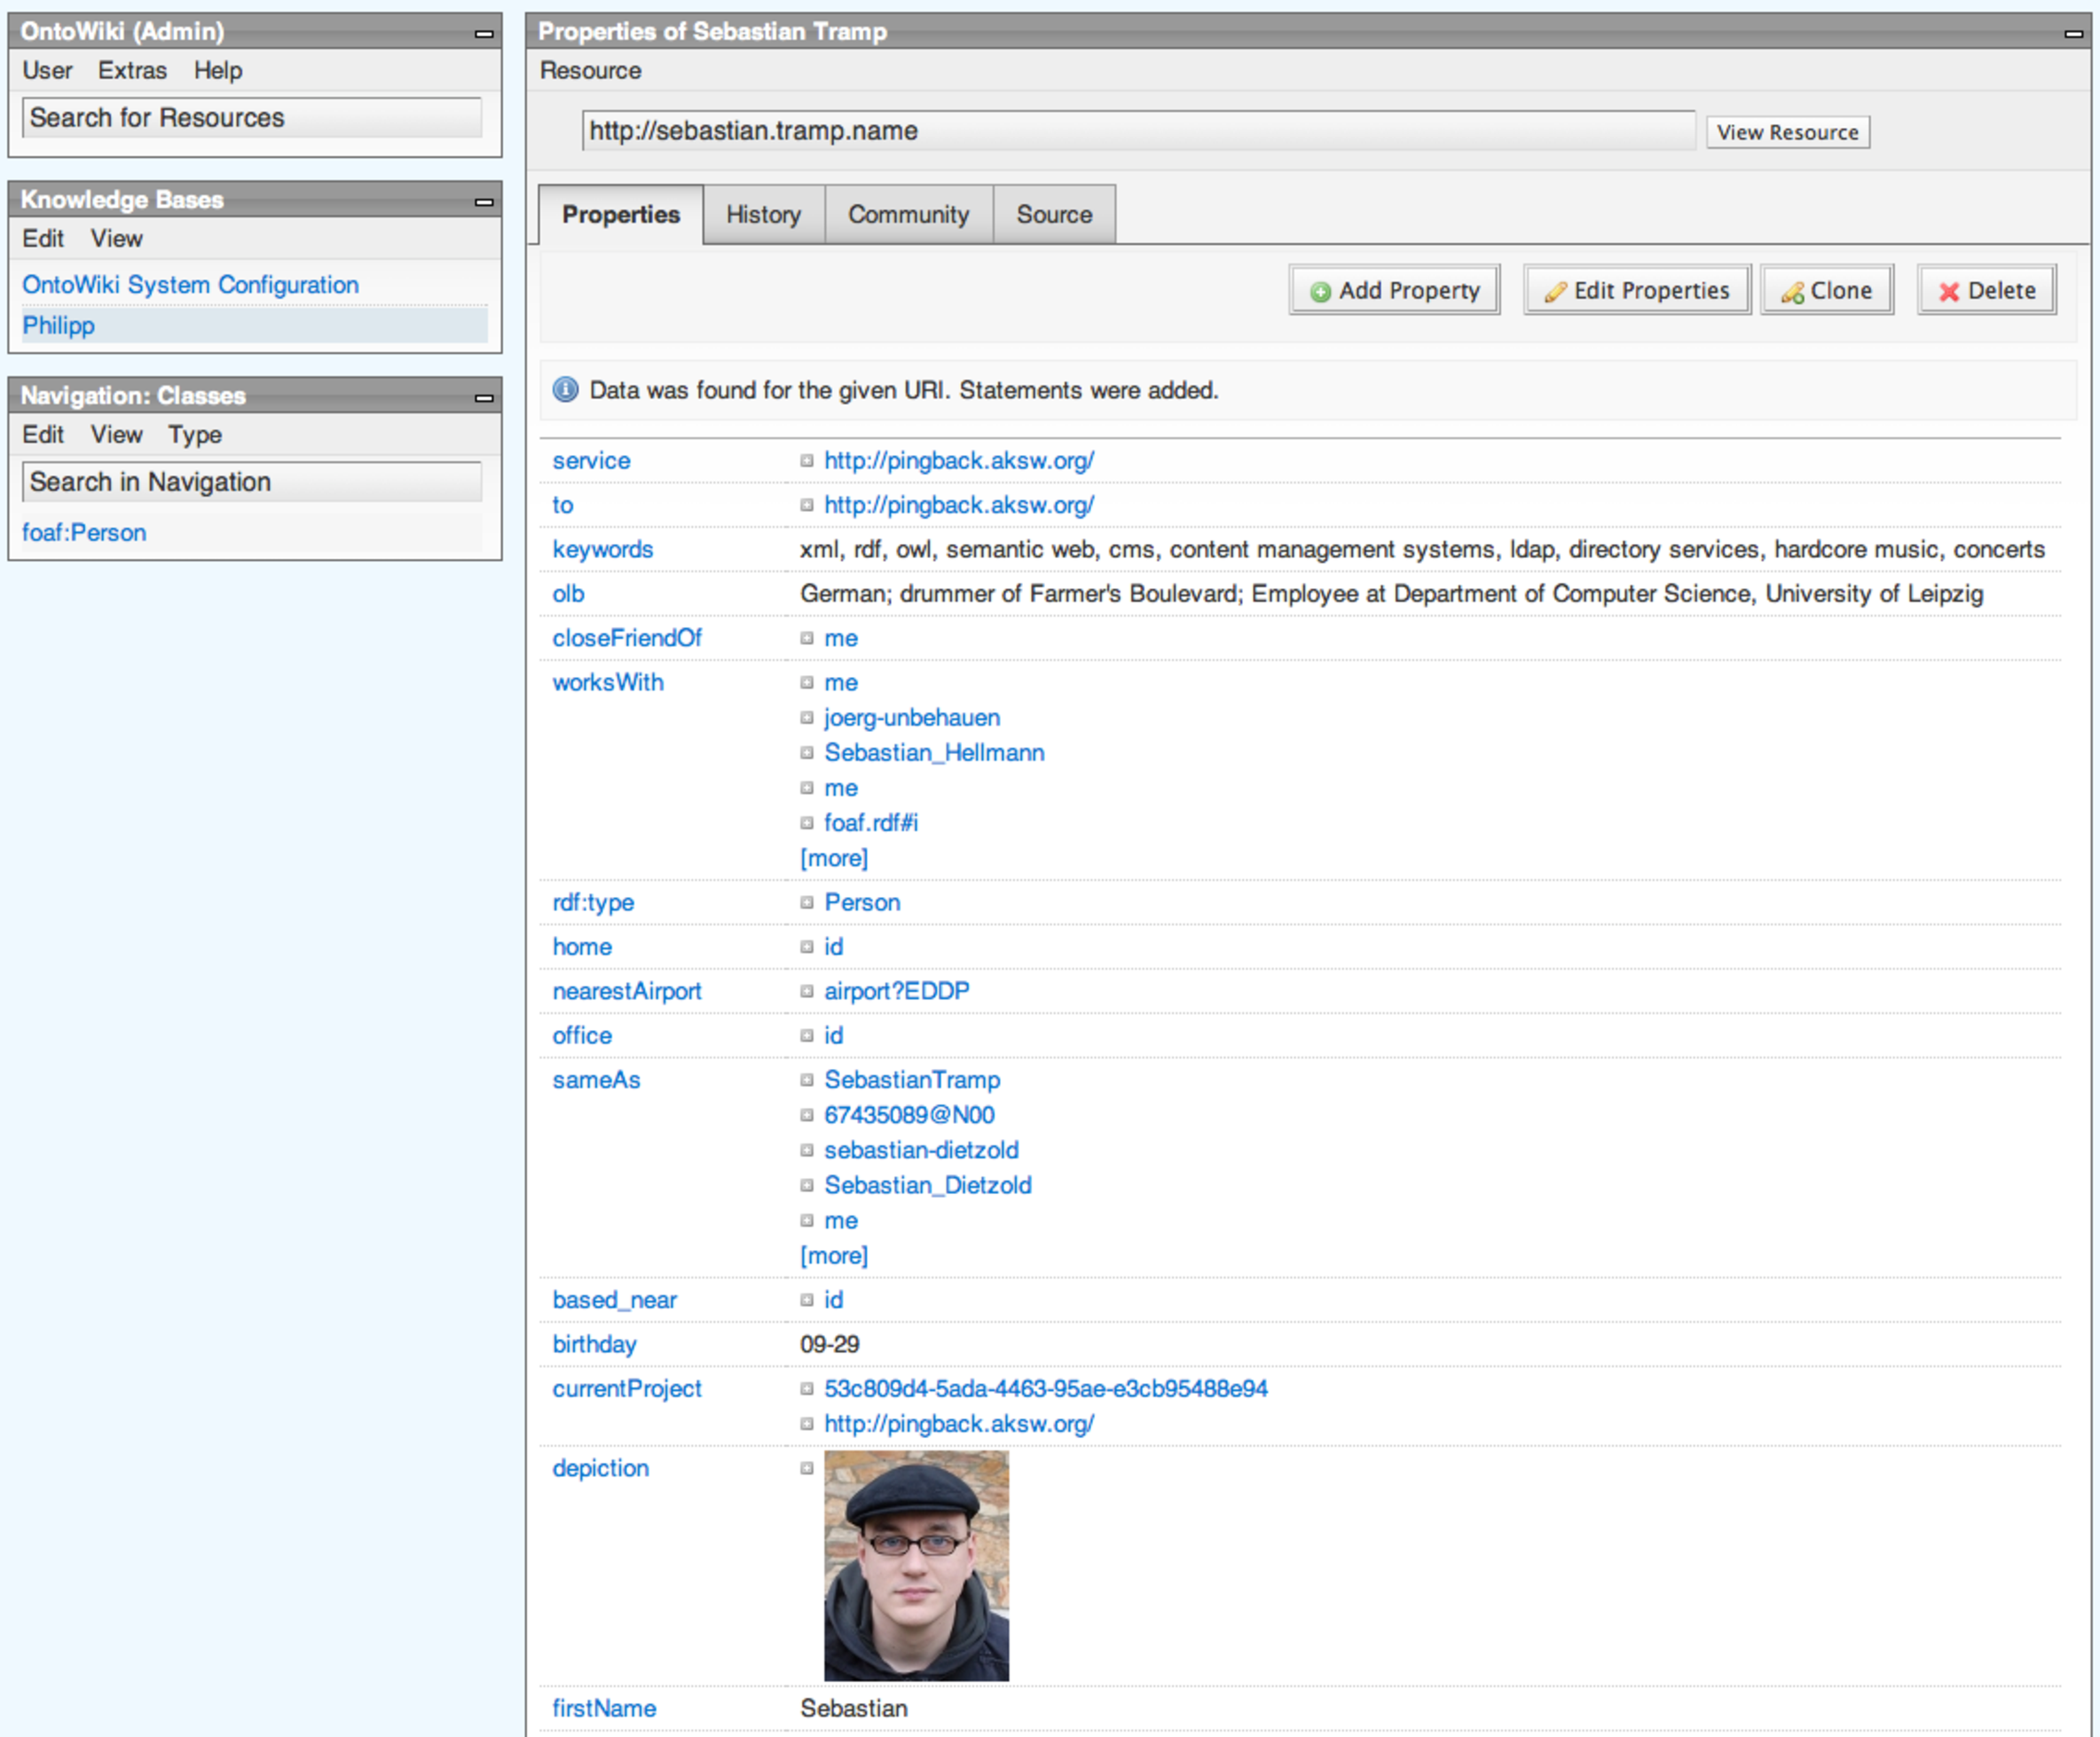
\includegraphics[width=\textwidth]{ontowiki}
  %\caption{An external and thus imported WebID profile shown in a generic OntoWiki view, which can be used to visualize arbitrary RDF resources.}
  %\label{fig:ontowiki}
%\end{figure*}

%\paragraph{Data import}
A first use-case for WebID access delegation within OntoWiki arises from an important functionality within OntoWiki, namely \textit{import of external data}.
%Figure \ref{fig:ontowiki} shows a WebID profile that was imported via the Linked Data principles into a local knowledge base.
Since WebID profiles can contain personal information that is in need of protection, access to such data should be restricted with the WebID protocol.
Although a user may (or may not in the case of a periodically executed automatic synchronization process) initiate the import procedure manually via the OntoWiki user interface, the actual fetching is done in the background.
An OntoWiki instance does not know of any private keys of users of the system.
Thus the system is not able to use that information when requesting data.
With WebID access delegation though, the profile can be fetched on behalf of the user instead.

%\paragraph{Semantic Pingback}
Another use-case where access delegation can be employed is within the \textit{Semantic Pingback} protocol~\cite{tramp-s-2010--b}.
With Semantic Pingback owners of resources can be notified when for example a link to such a resource is created elsewhere on the web.
In order to protect the protocol against spam attacks, a Pingback server will fetch the desired resource and check, whether the stated link is indeed contained in the data.
The source resource that links to the target resource and thus is fetched by a Pingback server might be access restricted, for example in a scenario where a friending process is initiated~\cite{story-h-2011--a}.
For privacy reasons the owner of the WebID profiles will very likely hide the triples in question (e.g. \texttt{foaf:knows}) on anonymous access attempts.
With WebID access delegation again, the resources can be fetched by the Pingback server on behalf of the resource owner.

This will require some further changes to the delegation protocol discussed up to now. 
Specifically the \lstinline|:secretary| relation currently does not distinguish what kind of repsonsibilities the \textit{principal} wishes to give to the \textit{secretary}. 
It is currently assumed that the secretary has full rights. For ontowiki knowing the social network may be all that is needed to make access control decisions. 
Full delegation powers may not be needed. The ability to describe more limited secretary relations could be very helpful here.

\section{Related Work}\label{sec:relatedwork}

%\subsection{OAuth}
\paragraph{OAuth~2.0}\cite{hardt-d-2012--a} is the latest version of the OAuth protocol, which is being presented as an access delegation protocol, enabling users to grant access to third-party services to their personal resources, instead of sharing their passwords with those third-party services.
OAuth includes two main parts: obtaining an access token by asking the resource owner (i.e. the user) to grant access, and then using the tokens to access protected resources. 
%Here is a typical example of using OAuth. 
%Ann has a Twitter account.
%One day she decides to support her favourite project by using Flattr\footnote{\url{http://flattr.com}}, a micro payment service.
%Since she would rather not create a new account, Flattr offers her the possibility of using her Twitter account to log into Flattr.
%After clicking the "Login using Twitter" button, she is redirected to Twitter's login page where she inputs her user name and password.
%Once authenticated, Twitter informs her that Flattr would like to access her personal information (e.g. name, picture, etc.).
%She can now choose if she wants to grant or deny to Flattr access to her Twitter account information.
%Once she accepts, she is redirected back to Flattr where she notices that she is now authenticated, and her Twitter user name, full name and picture now appear in Flattr.
The advantage here is that Ann only had to use her Twitter credentials to log into Flattr.  However, the disadvantage is that Flattr requires an existing trust relationship with Twitter, thus limiting the number of supported services.
Even if OAuth provides authentication as a by-product of having the resource owner authorize a third-party client to her resource server, its main focus is on resource authorization rather than on federated identity.
The conclusion is that OAuth is used to \textit{provide access for external services to local user resources} without disclosing the user's credentials.
%On the other hand, in WebID access delegation, the secretary is used to \textit{gain access to external resources} on behalf of a given user.
Or in other words: OAuth is used to allow an agent to \textit{request a users resources} while WebID delegation is used to allow an agent to \textit{request resources the user could request herself}.

\paragraph{Cross Origin Resource Sharing (CORS)}
In this paper we proposed to add an \lstinline|On-Behalf-Of| header to each HTTP request made by a \textit{secretary} in order to be able to identify the \textit{principal} she is working for in that particular request.
This is quite a major semantic addition to HTTP, but for which there is a widely adopted precedent, namely CORS\footnote{\url{http://www.w3.org/TR/cors/}}, the Cross Origin Resource Sharing spec at the W3C.
CORS identifies the remote \textit{principal} with an \lstinline|Origin| header, and uses any HTTP authentication method to identify the \textit{secretary} which is the browser.

Let us look at this in more detail.
CORS has two agents, one acting on behalf of the other, and these are: 
(1) The Browser: it takes the role of the \textit{secretary} as it is acting on behalf of javascript agents - the \textit{principals}.
(2) JavaScript code: hosted on the internet and identified by the Origin Server that hosted the javascript.
This javascript agent requests resources from the Browser, but it is unable to do it directly.

The use cases for CORS are slightly different from the ones for our delegation proposal. 
In CORS the browser is using its own identity credentials when connecting to remote servers (e.g. a bank), as it needs to alert the remote service that the request originates from a particular agent.
The browser also needs to make sure the remote server understands this, especially when authentication is required, to allow the remote server to evaluate the strength of the Javascript trust relation.
In the Section~\ref{sec:spec} use cases, the remote site trusts the \textit{principal}, but may not be aware of the \textit{secretary}.
In our proposal, the identification of the agent in the \lstinline|On-Behalf-Of| header is much more precise.
Combined with the ability of the secretary to also identify herself with a WebID, it builds an explicit trust relation between the \textit{principal} and the \textit{secretary}. The vagueness of the \lstinline|Origin| identity of the \textit{principal} in CORS makes a lot of this more difficult.

It is a topic of further research to evaluate in which circumstances it is important for the \lstinline|secretary| to also make sure that the remote server is aware that the connection being made is \lstinline|On-Behalf-Of| the specified \textit{principal}. 
For otherwise it is possible that the \textit{secretary} herself be made liable for the actions she is making on behalf of her \textit{principal}, especially were she to make \texttt{PUT}, \texttt{POST} or \texttt{DELETE} requests. 
The CORS protocol determines this by  requiring an initial \texttt{HEAD} request to a resource to be made, which will determine whether the server understands CORS.
With the help of TLS the server hosting the remote resource could have a WebID Profile describing it to be an understander of the \lstinline|On-Behalf-Of| header, makeing the protocol a lot more efficient and secure once more.

\section{Conclusion and Future Work}\label{sec:conclusion}

%\todo{Nice up wording esp. our terms and language}
In this paper we discussed different ways in which an agent, such as a Social Web application, can act on behalf of a user and request as well as manipulate resources on the Web in the name this user.
Our proposal for supporting such a communication schema involves an extension to the HTTP protocol, which allows for delegation of access authorization from one agent to another agent, both identified by their WebID.
The technical solution annotates these HTTP requests by adding the \lstinline|On-Behalf-Of| header field which refers to the WebID of the user in whose name the agent acts.
This distinguish the identities of the user and the agent and allows for creation of policy descriptions which use both WebIDs to specify the relations between the agent and the user in order to setup the access rules for this agent.
Since the protocol footprint is minimal, the main information entropy to decide whether an agent has the right to request a specific resource or not is available as part of the content of a WebID profile which can be requested as Linked Data.
We believe that such an shift of the entropy from a protocol endpoint (such as in OAuth) to a machine readable document is a crucial feature of Linked Data in general and WebID in detail.

However, at this point we postpone the answer to the question of how we should describe the access control rules in a users WebID profile.
There already exists first attempts from the Linked Data / Semantic Web and the Read Write Web communities such as the WebAccessControl vocabulary\footnote{\url{http://www.w3.org/wiki/WebAccessControl}}, $_{dg}$FOAF~\cite{schwagereit-f-2010-181-a} as well as different projects on policy creation and management~\cite{kagal-l-2005--a}.
In our future work we will try to close the gap between the policy and access control vocabularies on the one hand and WebID authentication on the other hand.
A rough abstract in which direction this should be elaborated is presented in \autoref{listing:views} and we hope that we can sensitize others to take up this challenge too.

\bibliographystyle{plain}
\bibliography{webid}

\end{document}
